\section{Specifications}

\subsection{Cardiac signal}

The electrical potentials of the cardiac signal are acquired by various electrodes conected in the surface of the skin of the patient. Those combined generate the cardiac signal, as can be seen in the normal wave pattern of figure \ref{fig:cardiac_signal}, with voltage differences in the order of $1 \, mV$ between given points in the body \cite{khandpur2019compendium}.

\begin{figure}[h!] 
    \centering
    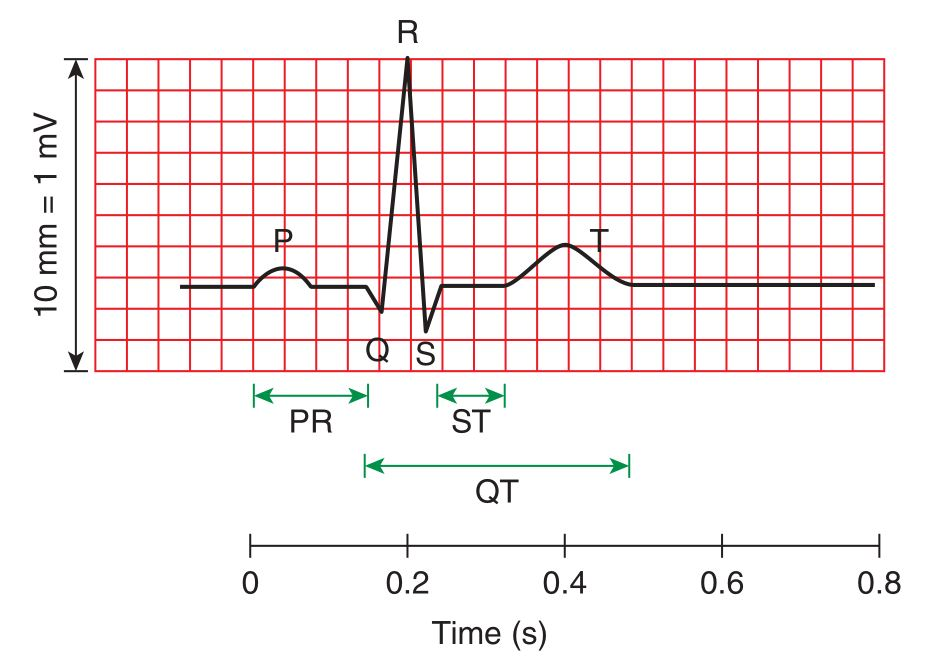
\includegraphics[width=9cm]{images/cardiac_signal.JPG}
    \caption{Normal waveform pattern of cardiac signal obtained in ECG. Source: \cite{khandpur2019compendium}.}
    \label{fig:cardiac_signal} 
\end{figure}

Regarding the figure \ref{fig:cardiac_signal}, each letter has a proper meaning for each step in the cardiac cycle. Those are:

\begin{itemize}
    \item The P wave represents the depolarization of the atrial muscles;
    \item The QRS section is a combination of the atria repolarization between QR and the ventricles depolarization between RS;
    \item The T wave represents de repolarization of both ventricles;
\end{itemize}

The interval PR represents the actrial systole, of which the diastole lasts from R until the next P wave. The ventricular systole occurs between R until the end of the T wave and its diastole lasts until Q \cite{openstax}. 

The interval QRS representing the time taken by the heart impulse to travel from the interventricular system then through the walls of the ventricles is the most critical one when thinking in the design of an ECG machine since it has the higher frequency of all the cardiac signal and lasts about 0.05 to 0.1 seconds \cite{khandpur2019compendium}.

\subsection{Associated noises}

\pagebreak